\documentclass[11pt, a4paper]{article}
%\DeclareUnicodeCharacter{200A}{!!!FIX ME!!!}

\usepackage[margin=1in]{geometry}
\usepackage{txfonts}
\usepackage{blindtext}
\usepackage{listings}
\usepackage{hyperref}
\usepackage{graphicx}
\usepackage{xcolor}
%\renewcommand{\lstlisting}{code}
\renewcommand{\lstlistlistingname}{List of codes}
\lstdefinestyle{chstyle}{%
backgroundcolor=\color{gray!12},
basicstyle=\ttfamily\small,
commentstyle=\color{green!60!black},
keywordstyle=\color{magenta},
stringstyle=\color{blue!50!red},
showstringspaces=false,
captionpos = b,
numbers = left,
numberstyle=\footnotesize\color{gray},
numbersep=10pt,
stepnumber=2,
tabsize = 3,
frame=L,
framerule=1pt,
rulecolor=\color{red},}


\title{C++ Tutorials for Beginners}
\author{Kouassi Franck Armand Prince
\date{09.05.2021}
}


\begin{document}

\maketitle\hrule
% \begin{center}
% \textbf{C++ Tutorials for Beginners}
% \end{center}
\newpage

\tableofcontents
\listoffigures
\lstlistoflistings
\pagebreak

\section{Getting Started}
%{\blindtext}
This section introduces the basics of C++ programming language and the tools
needed to follow this tutorial. The goal of this tutorial is to help beginners
getting started with C++ programming language. It does not require you to you to
have a prior programming background kownledge. All you have to do is to follow along
with me and and try to \textbf{\textit{WRITE}} the code on your own machine not just read.
Believe me it is easier to read and assume that you have mastered it until you are required
to write the code by yourself, that is where it realize you have not properly understood it.

\subsection{Understand the Computer Language}
%{\blindtext}
Your computer is an incredible and complicated device. Basically, the computer
understands one simple language composed of 0 and 1. Thus a message like this
"\textit{01001100101001010}" could mean "open a window" for instance. Fortunately, we do not have
to learn this language (Binary language). Programmers created languages which are much simpler
than binary language. Here you could check \href{https://en.wikipedia.org/wiki/List_of_programming_languages}
{\emph{\textit{the number of programming languages.}}} \newline
All programming languages have the same goal, that is being able to easily and efficently
communicate with the computer compare to binary language.\newline Here, is how it works :

1. You write the instructions to be executed by the computer in a programming language (e.g C++)

2. The instructions are translated in binary (0 and 1), the language understood by the computer.

3. The computer can now decode the message and executes your request.

\begin{figure}[!ht]
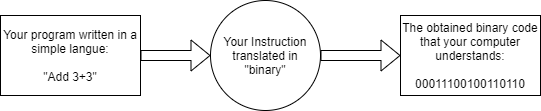
\includegraphics[width = \linewidth]{diagrams/compling.png}
\caption{Compliling Process.}
\label{fig:Compliling Process}
\end{figure}

\subsection{C++ against other programming languages}
% \subsubsection{sub sub section}
% {\blindtext}
% You might think of C++ as an antique programming language, but C++ is still readily used in programming today.
% Despite the advent of popular object-oriented programming languages like Python, C++ continues to have a dedicated
% space in the tech world.C++ is still the go to language for solutions that need fast machine performance. AAA video games, IoT,
% embedded systems, and resource-heavy VR and AI applications run on C or C++.
Before we start talking about why C++ reprsents a powerful language despite its age. let's discuss the
the key points to analyze before diving into a language.

There exists numerous programming languages as mentioned in above section, although some languages are interesting, 
they are seldom used. The main challenge that comes with these languges, is that they do not have a very big community 
so imagine you working on a project and you are facing a problem, it is difficult to find help since not so many people 
are using the the language.This explains why C++ represents a good choice for debutant programmers. You are not alone, a lot
ressources are availble to guide through your learning process, also C++ is still being widely used.

Another interesting aspect to look at as well is the programming language level. There are of two (02)
types: \textbf{\textit{{high level}}} and \textbf{\textit{{low level}}}.
\newline
\textbf{\textit{{high level}}}: is a language that is that is far from binary language and really
to humans languge,it allows to easily understand and translate instructions contrary to \textbf{\textit{{low level}}}
which a language closed to machine language and generally requires much more effort but gives you more 
control over what you can do, it is a trade-off.

\begin{figure}[h!]
    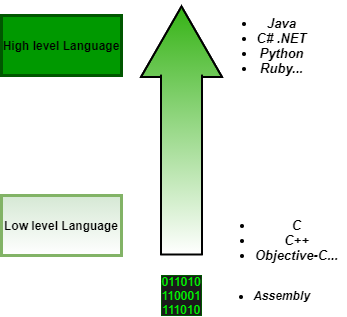
\includegraphics[width = \linewidth]{diagrams/low vs high.png}
    \caption{Programming Language by level.}
    \label{fig:Programming Language by level}
\end{figure}
C++ is a low level language. Do not panic, although coding in C++ might be a little complex, you will 
have in your possession a very \textbf{\textit{{powerful}}} and particulary \textbf{\textit{{fast}}} language.
Infact, if most games are developed in C++, it is because it is the language capable of coupling
speed and power, that makes it an essential language.



\subsection{Summary of C++}
Here we are going to showcase some aspects of C++ that make it an important language regardless of
how long it has been since it creation.
\begin{itemize}
    \item \textbf{Popularity} : C++ is one of the most popular
    languages in the world. It is used by some 4.4 million developers worldwide
    \item \textbf{Large Community} : There is a large online community
    of C++ users and experts that is particularly helpful in case any support is required.
    There is a lot of resources available on the internet regarding C++.
    \item \textbf{Portable} : Programs developed in C++ can be moved from one platform
    to another. This is one of the main reasons that applications requiring multi-platform
    or multi-device development often use C++.
    \item  \textbf{Speed} : Programs written in C++ language execute more faster compare
    to most programming languages\end{itemize}

\paragraph{Snippet of C++}
To give you an idea of how the code looks, let's look at a simple C++ program displaying "Hello world!"
on the screen. Do not try to understand the code just appreciate the beauty and structure. We will
go into details in the following sections

\begin{lstlisting}[caption=Sample example of C++ programming language, style=chstyle, language=C++]
//=================================================
// Sample example of C++ programming language
//=================================================

#include <iostream>

using namespace std;

int main()
{
    cout << "Hello world!" << endl;
    return 0;
}
//=================================================
\end{lstlisting}
\textit{ If you are interested in knowing the story of C++ starting from its creation,
\href{https://en.wikipedia.org/wiki/Bjarne_Stroustrup}{you can learn all about C++ from wikipedia}}

\subsection{Summary}
% \subparagraph{sub paragraph}
% {\blindtext}
\begin{itemize}
    \item Programs allow us to efficently control actions on the computer: web browsing, text editing etc
    \item In order to create a program, we write instructions for the computer using a programming; source code
    \item The source code must be converted in binary by what we could a compiler, it allows the executation 
    of the code.
    \item  C++ is a widely used programming language, it is an evolution of C programming due to the fact that 
    it allows Object Oriented Programming (OOP), a very powerful programming feature.
\end{itemize}
\newpage

\section{Environment setup}
In this section, we are going to introduce the tools needed to follow
this tutorial.From our previous discuss, you already know by now an important
tool needed, Yes you are right, you need a Compiler, the program that
converts your C++ code into the computer readable format.

Aside these, there are additional tools needed for you to code with ease
\begin{itemize}
    \item \textbf{A text editor}: It will allow you to write your source
    code. On windows we have Notepad or Vi on linux. But of course, it is
    less recommed because as your code gets bigger and bigger, you might not 
    not be  able to fully control it.
    \item \textbf{A compiler}: as mentioned above, it converts your source code into
    binary format for the computer
    \item \textbf{A debugger}: it helps you find bugs in your programs.
\end{itemize}
From now on we have two options (02) either we get the programs seperatly
which is of course much complicated, but on Linux most programmers prefer 
to use them in that way, I will not go into much details here, instead we 
are going to explore the simple way. We can get a program "3 in 1",
Yes you heard me correctly, a tool capable of handling the 3 listed tools 
It is commonly refered to as an \textbf{IDE} (Integrated Developement Environment).
There are of numerous types. In this tutorial we are not going to discuss 
their similarities. I personnaly recommed Visual Studio Code and here is
how you can \href{https://code.visualstudio.com/docs/languages/cpp}
{get started with C++ for Visual Studio Code}. So go ahead and install the
necessary packages.

\section{Your first C++ code}



































\end{document}